\section{Theoretische Grundlage}
\label{sec:Theorie}
\subsection{Ziel}
Ziel des Versuches ist es der elastisches Modul eines Metalls mittels einer Drehschwingung zu bestimmten, als auch das magnetische Moment eines Permanentmagneten.
\subsection{Normal-, Schubspannung und Hooksches Gesetz}
Kräfte die an die Oberfläche eines elastischen Körper angreifen, verformen diesen. Aufgrund dessen werden die Größe Spannung definiert, welche ein Verhältniss von der Kraft zum ein Flächenelement herstellt.
\begin{equation}
  \sigma = \frac{F}{m^2} \, \frac{\text{N}}{m^2}
  \label{eqn:Spannung}
\end{equation}
Sie lassen sich in zwei Kategorien aufteilen. Als Normalspannung $\sigma_\text{N}$ werden die Kräfte bezeichnet welche senkrecht zur Oberfläche stehen. Die Kräfte welche parallel zur Oberfläche stehen heißen Schubspannung $\sigma_\text{S}$. Desweiteren gibt es noch Volumenkräfte. Bei solchen greift die Kraft an jedem Volumenelement an, zum Beispiel die Schwerkraft.

Zwischen hinreichend kleinen Spannungen und Deformation besteht ein proportionaler Zusammenhang welcher als Hooksches bezeichnet wird.
\begin{equation}
  \sigma = E \frac{\Delta L}{L}  \hspace{2em} \text{und} \hspace{2em} P = Q\frac{\Delta V}{V}
  \label{eqn:Hook}
\end{equation}
Um alle Spannungen in einem Kristall volständig zu beschreiben werden jeweils 6 Komponenten benötigt, wobei 3 für die Gestaltsund 3 für die Volumenelastizität zuständig sind. Bei einem einfachen  Kristall mit niedriger Symmetrie entsteht deswegen eine 6x6-Matrix mit 36 Einträgen. Bei kubischen Kristallen lässt sich aufgrund der symmetrie der Matrix und des Körpers auf 3 Einträge verringern.

\subsection{Elastische Konstanten isotroper Stoffe}
Zur Berechnung des elastizitschen Konstanten wird einerseits die Torsionsmodul $G$ als auch das Komprssionsmodul $Q$ benötigt bzw das Elastizitätsmodul $\sigma$.
Die Poissonsche Querkontraktionszahl µ Verknüpft die Längenänderung mit der Normalspannung. Die Abbildung \ref{fig:poisson} soll die anhand eines einseitig eingespannten Stab verdeulichen.
\begin{figure}
  \centering
  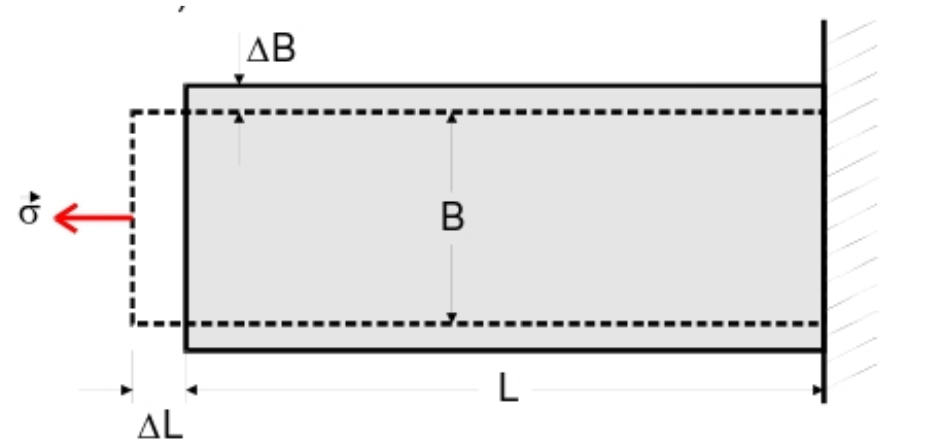
\includegraphics[width=5.0cm]{./picture/poisson.png}
  \caption{<+caption text+>}
  \label{fig:poisson}
\end{figure}
\begin{equation}
  µ := -\frac{\Delta B}{B} \cdot \frac{L}{\Delta L}
  \label{eqn:pois}
\end{equation}


\subsection{Fehlerrechnung}
\subsubsection{Mittelwert}
Der Mittelwert einer Messreihe $x_\text{1}, ... ,x_\text{n}$ lässt sich durch die Formel
\begin{equation}
	\overline{x} = \frac{1}{N} \sum_{\text{k}=1}^\text{N} x_k
	\label{eqn:ave}
\end{equation}
berechnen. Die Standardabweichung des Mittelwertes beträgt
\begin{equation}
	\Delta \overline{x} = \sqrt{ \frac{1}{N(N-1)} \sum_{\text{k}=1}^\text{N} (x_\text{k} - \overline{x})^2}
	\label{eqn:std}
\end{equation}

\subsubsection{Fehlerfortpflanzung}
Die Fehlerfortpflanzung übernimmt Python 3.4.3 mit der Funktion "ufloat" aus "Python-Uncertainties".

\subsubsection{Lineare Regression}
Die Lineare Regression und sämtliche andere Rechnungen wurden ebenfalls mit Python 3.4.3 durchgeführt.
